\chapter{Natural Language Processing (NLP)}

Natural Language Processing (NLP) is a subfield of artificial intelligence that focuses on the interaction between computers and humans through natural language. The ultimate objective of NLP is to enable computers to understand, interpret, and generate human language in a way that is both meaningful and useful. It is a multidisciplinary field that combines linguistics, computer science, and machine learning to process and analyze large amounts of natural language data. Some of its difficulties include:
\begin{itemize}
    \item Ambiguity: Words and sentences can have multiple meanings depending on the context.
    \item Variability: Different people may express the same idea in different ways.
    \item Complexity: Natural language is inherently complex, with intricate grammar and syntax rules.
    \item Data Sparsity: There may be limited data available for certain languages or dialects.
\end{itemize}

\section{Linguistic Analysis}

Linguistic analysis in NLP involves examining the structure and meaning of language. In order to do so, several approaches can be employed.

\subsection{Structural Analysis}

Structural analysis focuses on the syntax and grammar of language. It involves breaking down sentences and tagging the different parts. Two main techniques used in structural analysis are:
\begin{itemize}
    \item Part-of-Speech (POS) Tagging: This technique involves labeling each word in a sentence with its corresponding part of speech, such as noun, verb, adjective, etc.
    \item Named Entity Recognition (NER): This technique identifies and classifies named entities in text, such as names of people, organizations, locations, dates, etc.
\end{itemize}

The problem of structural analysis is that it can be challenging to accurately parse sentences, and it is usually really slow.

\subsection{Statistical Analysis}

Statistical analysis in NLP involves using statistical methods to analyze and model language data. They depend on the \emph{Corpus} considered, which is a large and structured set of texts that can be used for training and testing NLP models. Some common aspects that are taken into account in statistical analysis include:
\begin{itemize}
    \item \ul{Letter Frequency}: This involves analyzing the frequency of a letter in a language.
    \item \ul{Start and End of Word}: This involves analyzing the frequency of letters at the start and end of words.
    \item \ul{N-grams}: This involves analyzing the frequency of sequences of $n$ letters or words in a language.
\end{itemize}

Taking statistical analysis into account, the following laws were formulated:
\begin{itemize}
    \item \ul{Zipf's Law}: This law states that the frequency of a word is inversely proportional to its rank in the frequency table. In other words, the most frequent word will occur approximately twice as often as the second most frequent word, three times as often as the third most frequent word, and so on. It can be expressed mathematically as:
    \begin{equation}
        f(r) = \frac{C}{r^s}
    \end{equation}
    where $f(r)$ is the frequency of the word with rank $r$, $C$ is a constant, and $s\approx 1$ is a parameter that determines the slope of the distribution.

    \item \ul{Heaps' Law}: This law describes the relationship between the size of a vocabulary and the size of a corpus. It states that as the size of a corpus increases, the size of the vocabulary also increases, but at a slower rate. It can be expressed mathematically as:
    \begin{equation}
        V(n) = K n^\beta
    \end{equation}
    where $V(n)$ is the size of the vocabulary, $n$ is the size of the corpus, $K$ is a constant, and $\beta$ is a parameter that determines the rate of growth of the vocabulary (usually $\beta\in \left[0.4, 0.6\right]$).
\end{itemize}

These laws are important in NLP, because they allow users to distinguish real and generated texts, and they can be used to improve the performance of NLP models by providing insights into the structure and distribution of language data.

\section{Text Processing Pipeline}

The text processing pipeline is a series of steps that are applied to raw text data to convert it into a format suitable for machine learning algorithms. During the following sections, we will discuss the main steps of the text processing pipeline.

\subsection{Tokenization}

Tokenization is the process of breaking down a text into smaller units called tokens. Tokens can be words, phrases, or even individual characters. 

\subsection{Normalization}

Normalization is the process of converting text into a standard format. This can involve several steps, such as:
\begin{itemize}
    \item Lowercasing: Converting all text to lowercase to ensure uniformity.
    \item Removing Punctuation: Eliminating punctuation marks from the text.
    \item Removing Special Characters: Eliminating special characters, such as emojis or symbols, that may not be relevant for analysis.
    \item Expanding Contractions: Converting contractions (e.g., ``can't'') into their expanded forms (e.g., ``cannot'').
\end{itemize}

\subsection{Stemming or Lemmatization}

Stemming and lemmatization are techniques used to reduce words to their base or root form.
\begin{itemize}
    \item \ul{Stemming}: This technique removes suffixes from words to obtain their root form (which sometimes may not be a valid word). It is simple and fast, but it can lead to errors.
    \item \ul{Lemmatization}: This technique reduces words to their base or dictionary form (which is always a valid word). It is more accurate than stemming, but it can be slower and more complex.
\end{itemize}

\subsection{Stop Words Removal}

Stop words are common words that do not carry significant meaning and are often removed from text data to improve the performance of NLP models. Examples of stop words include ``the'', ``is'', ``in'', ``and'', etc. Removing stop words can help reduce noise in the data and improve the accuracy of NLP models. However, this step should be done carefully, as some stop words may carry important meaning in certain contexts.

\subsection{Feature Extraction}

After preprocessing the text data, the next step is to extract features that can be used as input for machine learning algorithms. Feature extraction involves transforming the text data into a numerical representation that can be processed by algorithms.

\subsubsection{Bag of Words (BoW)}

The Bag of Words (BoW) model creates a vocabulary of all unique words in the corpus and represents each document as a vector of word frequencies. Therefore, the order of words is ignored.

\subsubsection{Term Frequency-Inverse Document Frequency (TF-IDF)}

The Term Frequency-Inverse Document Frequency (TF-IDF) model is a statistical measure that evaluates the importance of a word in a document relative to a corpus. It consideres two components:
\begin{itemize}
    \item \ul{Term Frequency (TF)}: This measures how frequently a term appears in a document. It is calculated as:
    \begin{equation}
        TF(t,d) = \frac{f_{t,d}}{\sum\limits_{t' \in d} f_{t',d}}
    \end{equation}
    where $f_{t,d}$ is the frequency of term $t$ in document $d$.
    \item \ul{Inverse Document Frequency (IDF)}: This measures how important a term is in the entire corpus. It is calculated as:
    \begin{equation}
        IDF(t,d) = \log\frac{N}{n_t}
    \end{equation}
    where $N$ is the total number of documents in the corpus, and $n_t$ is the number of documents containing term $t$.
\end{itemize}

The TF-IDF score is then calculated as the product of TF and IDF:
\begin{equation}
    TF-IDF(t,d) = TF(t,d) \cdot IDF(t,d)
\end{equation}

\subsubsection{Word Embeddings}

Word embeddings are dense vector representations of words that capture semantic meaning and relationships between words. Similar words are represented by similar vectors in the embedding space, so they can be used to capture the meaning of words in context.

\section{Transformers}

\begin{observacion}
    This section is based on the article \myhref{https://arxiv.org/pdf/1706.03762}{Attention Is All You Need}, which introduces the Transformer model. For further information, please refer to the original article.
\end{observacion}
\begin{figure}
    \centering
    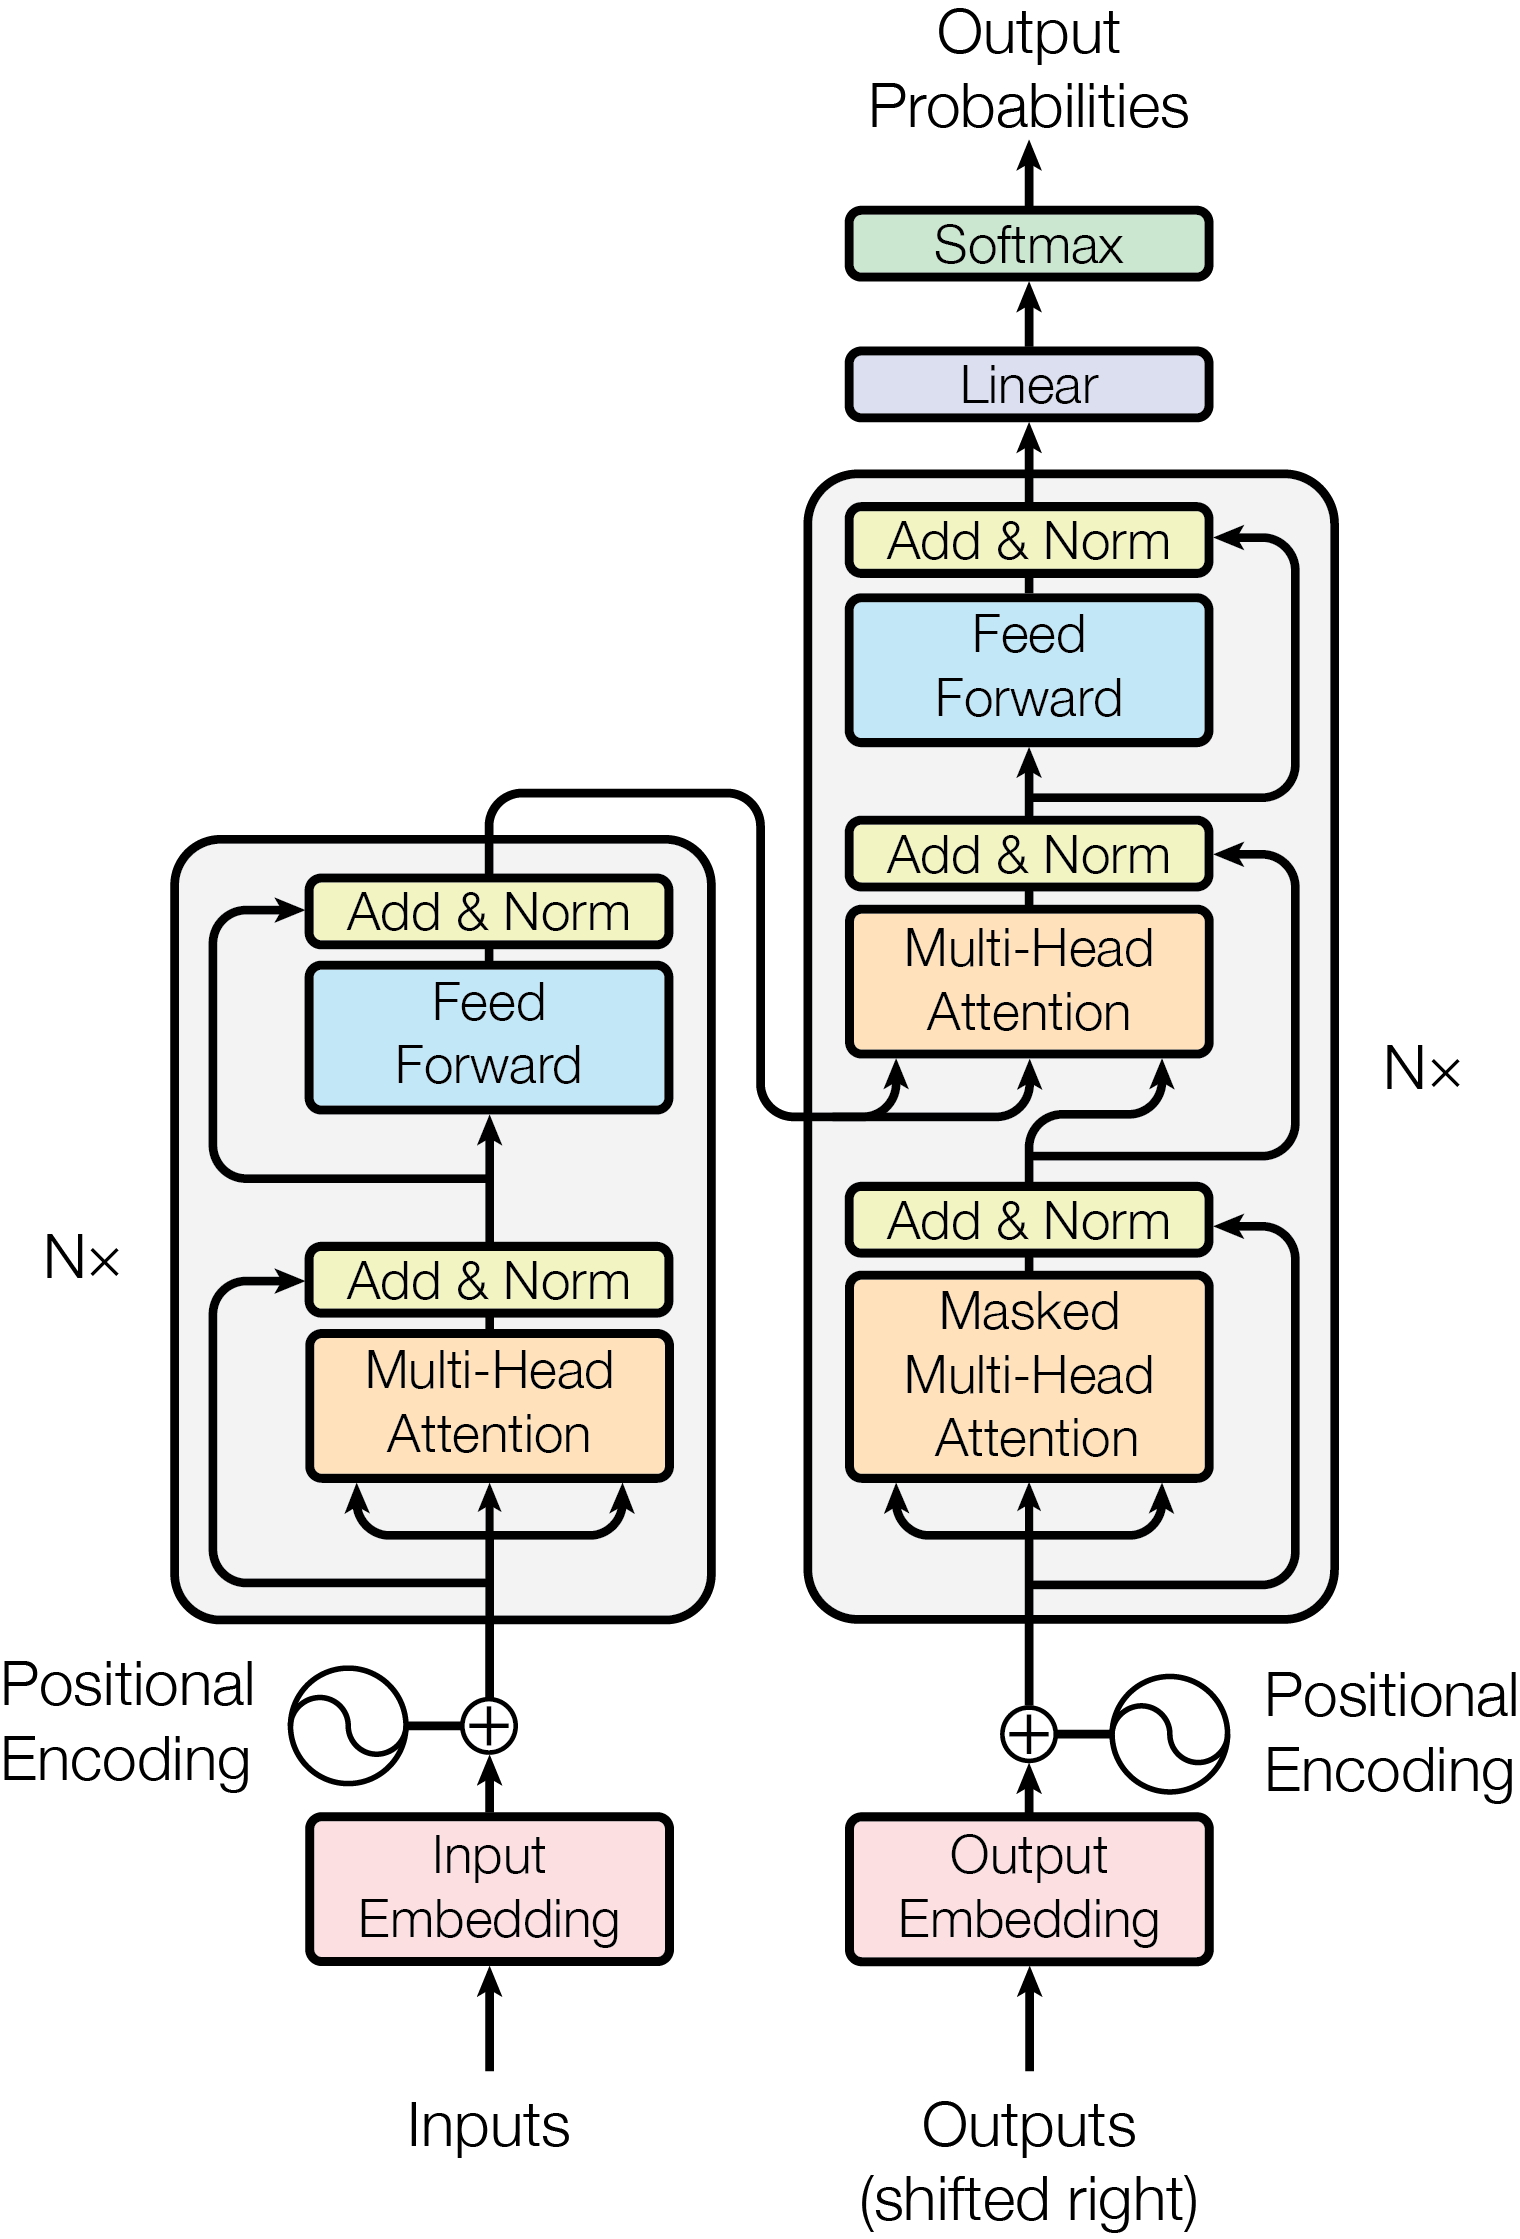
\includegraphics[width=0.7\textwidth]{images/Transformer.png}
    \caption{The architecture of the Transformer model.}
    \label{fig:transformer}
\end{figure}

The architecture of the Transformer model (see Figure \ref{fig:transformer}) has two main components:
\begin{itemize}
    \item \ul{Encoder}: The encoder takes the input sequence and processes it to generate a set of hidden representations.
    \item \ul{Decoder}: The decoder takes the hidden representations generated by the encoder and the previous output sequence to generate the next\footnote{Even though the encoder processes the whole input at a time, the decoder generates one element at a time. In addition, it is auto-regressive.} token in the output sequence.
\end{itemize}

For each input (both the inputs for the encoder and the previous outputs for the decoder), word embeddings are generated to convert the input tokens into dense vector representations. The position of each token in the sequence is also encoded, so that the model can take into account the order of the tokens.

The Transformer model uses a mechanism called \emph{self-attention} to capture the relationships between tokens in the input sequence. Therefore, the model can focus on different parts of the input sequence when generating the output sequence.

Lastly, a Large Language Model (LLM) is a type of neural network based on the Transformer architecture that is trained on really large corpora of text data. LLMs are capable of generating human-like text and performing a wide range of NLP tasks, such as text classification, question answering, and language translation.